\subsection{Evaluation}\label{sec:evaluation}

In the following sections, we evaluate the implemented system. We compare our implementation of the system against the system requirements established in Section~\ref{sec:system-reqs} (p. \pageref{sec:system-reqs}) and then compare individual system components against their respective requirements (Section~\ref{sec:component-reqs}, p. \pageref{sec:component-reqs}). For every requirement we review, whether it was implemented fully, partially or not at all and asses, what implications does not implementing this requirement have on the overall system. Afterwards, a model transaction will be performed on test networks, using two Android devices.

\subsubsection{Requirement implementation evaluation}

We were able to implement all of the functional and two non-functional system requirements. We did not succeed in fully implementing one non-functional requirement -- PT-NFR-2 in particular. This requirement specifies that there should not be a single point of failure in the system. There are several places in the system, where this requirement is not adhered to. The prototype application only communicates with one single Ethereum node (single Infura instance), the deployed smart contract only contacts one oracle (Oraclize) and the oracle only contacts one blockchain explorer service (Blockchain.info). If any of these providers went offline, the system could not make transactions. Table~\ref{tab:system-reqs-eval} provides an overview over system requirements. Similar table elaborating on requirements of individual system components can be found in Appendix~\ref{sec:appendix-table} (p. \pageref{sec:appendix-table}).

\begin{table}[ht]
    \centering
    \begin{tabularx}{\textwidth}{|l X c|}
    \hline
    \textbf{ID}&\textbf{Description}&\textbf{Implemented}\\
    \multicolumn{3}{|l|}{\textbf{Functional requirements}}\\
    PT-FR-1 & The primary user and the secondary user should be able to agree on the terms of the transaction.&Yes\\
    PT-FR-2 & The primary user must be able to deploy a smart contract to the Ethereum network.&Yes\\
    PT-FR-3 & The secondary user should be able to verify contract deployment.&Yes\\
    PT-FR-4 & The secondary user should be able to transfer Bitcoin.&Yes\\
    PT-FR-5 & If the secondary user does not transfer Bitcoin, the primary user must receive their Ether back.&Yes\\
    PT-FR-6 & Primary user and secondary user must be ably to verify the status of their transaction.&Yes\\
    \multicolumn{3}{|l|}{\textbf{Non-functional requirements}}\\
    PT-NFR-1&The system must implement architecture proposed in Figure~\ref{fig:arch-ver2-tech}.&Yes\\
    PT-NFR-2&There should not be single point of failure in the system.&\textbf{No}\\
    PT-NFR-3&No other party should have control over the funds of primary user and secondary user.&Yes\\
    \hline
    \end{tabularx}
    \caption{Overview over system requirements. One requirement was not successfully implemented.}
    \label{tab:system-reqs-eval}
\end{table}

Ideally, the application would have a list of back-up nodes which it can contact in case that the primary node is unresponsive. Furthermore, the application should consult these back-up nodes to verify, that the primary node deployed the transaction to the network. The back-up nodes should be from different providers and preferably hosted at different locations. Only this way, the users can be certain that there is no single party having influence over these nodes. This requirement was not implemented in the first version of the system due to technical challenges and costs associated with deploying and/or connecting to a series of Ethereum nodes and due to the fact, that the idea initial can be successfully demonstrated with single Ethereum node. Non-functional requirements EN-NFR-1, EN-NFR-2 and EN-NFR-3, which specify the performance of the Ethereum node in terms of honesty and trustworthiness are not marked as \textit{Fulfilled}, since it is not possible to enforce these qualities in a single node. If a solution with back-up nodes was implemented, these requirements would not be relevant anymore.

Similarly, the smart contract only queries one oracle (Oraclize) and this oracle queries one blockchain explorer (Blockchain.info). If either the oracle or the blockchain explorer goes offline or deliberately provides incorrect responses, the transaction would not execute correctly. Neither the oracle nor the blockchain explorer do not directly control user's funds, but if they deliberately provided a false answer to the smart contract (e.g stating that the balance on the queried address is higher than it actually is), the transaction would not execute correctly. In the given example, the secondary user would receive Ether from the smart contract, even though they did not uphold their part of the agreement and did not transfer the Bitcoins. Ideally, to remove dependency on a single provider, the smart contract should query several independent oracles, with a different blockchain explorer as the target in every query. In case different responses are received, smart contract would need to decide which response to pick as the correct one (probably the most common one). If this was the case, requirements OR-NFR-1, OR-NFR-2, BE-NFR-1 and BE-NFR-2 would lose their relevance.

The prototype version of the system does not implement this, as currently there are not enough providers offering services of an oracle, that could be used. Some competitors of Oraclize either went out of business (case of Tinypay.co\footnote{\url{https://medium.com/@mustwin/building-an-oracle-for-an-ethereum-contract-6096d3e39551}, accessed 19-05-2018}) or do not offer the desired functionality -- contacting a web API (case of RealityCheck\footnote{\url{https://github.com/realitykeys/realitycheck}, accessed 19-05-2018}). We did not attempt to deploy our own oracle, as this is not the scope of this project.

Another requirement which was not fully implemented is the requirement SC-NFR-2, which states that smart contract must cover the costs for the services of the oracle. This requirement is not relevant in current implementation, as Oraclize does not charge any fees for the first query made from a smart contract. Since a new smart contract is deployed with every transaction and with current system there is only one query made right after the contract was created, no fees for the oracle are needed. However, if Oraclize changed their fees or if another provider was used, smart contract would need to be adapted for this.

Last requirement which was not implemented is the requirement CB-NFR-1. This is marked as \textit{Not implemented}, because in the prototype, users are not able to proceed with the transaction, unless the transaction status code has been update in the database. The current prototype does not accommodate users that agree on the terms of the transaction via another channel than the application itself. This behaviour could be easily changed by adapting the user interface of the application and allowing user to proceed with the transaction without consulting the transaction progress with the database.
%
%
%
%
%
%%%%%%%%%%%%%%%%%%%%%%%%%%%%%%%%%%%%%%%%%%%%%%%%%%%%%%%%%%%%%%%%%%%%%%%%%%
\subsubsection{Example of a transaction scenario}
In this experiment we demonstrate a transaction between two fictitious people -- a primary user Eve, who wants to sell Ether and buy Bitcoin, and secondary user Mike, who wants to buy Ether and sell Bitcoin. Both users are running the application on their phones. Eve has her own Ethereum wallet with some Ether she wishes to sell. Mike has his own Bitcoin wallet he will use to make the transaction. Eve's and Mike's wallets are standalone systems, independent from our system. The scenario of the transaction is outlined in Figure~\ref{fig:transaction-scenario}. 

\begin{figure}[ht]
    \centering
    \begin{framed}
    \begin{enumerate}[noitemsep]
        \item Mike creates a Bitcoin offer in the application by inputting:
            \begin{itemize}[nolistsep,noitemsep]
                \item Amount in Bitcoin he wishes to sell.
                \item Amount in Ether he wishes to receive.
                \item Ethereum address, where he wishes to receive the Ether.
            \end{itemize}
            Mike then and publishes this offer in the database.
        \item Eve selects this offer and transfers Ether to a temporary Ethereum address.
        \item Eve then creates an empty Bitcoin address and inputs this address into the application.
        \item A smart contract is deployed from the temporary address with following properties:
            \begin{itemize}[nolistsep,noitemsep]
                \item Mike's Ethereum address.
                \item Eve's Bitcoin address.
                \item Amount of Bitcoin, Eve and Mike are trading.
            \end{itemize}
            Besides these properties, which are specified in the smart contract constructor as data fields, the creation of a contract also carries two other significant information:
            \begin{itemize}[nolistsep,noitemsep]
                \item Sender's Ethereum address -- this is used to return the funds in case of unsuccessful transaction.
                \item Value, associated with the transaction -- this is the amount of Ether that Eve and Mike are trading.
            \end{itemize}
        \item After the smart contract has been deployed, Mike verifies correctness of the information in it. If all information are correct, Mike transfers Bitcoin to Eve.
        \item The oracle responds to a query sent by smart contract. Based on this response, smart contract sends its Ether balance either to Mike (in case of successful transaction) or to Eve (in case of unsuccessful transaction).
    \end{enumerate}
    \end{framed}
    \caption{Scenario of a transaction between Eve and Mike.}
    \label{fig:transaction-scenario}
\end{figure}

We successfully executed this scenario using two Android devices, a Parity Ethereum wallet and a GreenAddress Bitcoin wallet. The transactions were made on Ethereum \textit{Kovan} test network and Bitcoin \textit{testnet3} test networks. Eve's device was a OnePlus A5000 running Android 8.1.0 Oreo. Mike's device was a Samsung AM-A510F, running Android 7.0.0 Nougat. Both devices were connected to a mobile network and were sharing their screens with a computer via \acrshort{adb}. The whole process took approximately 20 minutes, out of which 10 minutes is the oracle response delay. The cost of the smart contract deployment was approximately 0.05 kETH\footnote{\textit{kETH} is used to indicate Kovan Ether.} and was paid by Eve\footnotemark. Table~\ref{tab:trade-story} describes the experiment progress step-by-step. Figure~\ref{fig:screenshot-contract} (p. \pageref{fig:screenshot-contract}) shows the application screen after the smart contract has been sent to the network. In Appendix~\ref{sec:appendix-screenshots} (p. \pageref{sec:appendix-screenshots}) we include complete list of screenshots taken during the experiment and their description. We can conclude, that successful execution of this scenario proves, that the proposed system is operational and can be used for~its~purpose.
% 
\footnotetext{We elaborate further on the cost of the transaction in the Discussion chapter (p. \pageref{sec:discussion}.)}

\newgeometry{left=0.5cm,right=.5cm,top=.5cm,bottom=1cm,footskip=.4cm}
\begin{table}[ht]
    \centering
    \begin{tabularx}{\textwidth}{|c|X|X|}
        \hline
        \textbf{Step}&\textbf{Eve}&\textbf{Mike}\\
        \hline
        1&Opens the application.&Opens the application.\\
        \hline
        2&Sees, that there are currently no available offers.&Clicks on \textit{Create new offer}.\\
        \hline
        3&&Fills in the amount of Bitcoin he wishes sell and amount of Ether he wishes to buy.\\
        \hline
        4&&Uses QR code scanner to input the address of his Ethereum wallet.\\
        \hline
        5&&Clicks on \textit{Create new offer}. This sends the offer to the database.\\
        \hline
        6&A new offer is added to the list. Eve selects this offer and clicks \textit{Confirm}.&Is presented with a screen showing the status of his offer.\\
        \hline
        7&A temporary address, from which the contract will be deployed, is presented to Eve. She has a choice to use this temporary address or import her own. She decides to use the temporary address.&\\
        \hline
        8&She transfers the amount of Ether to sell to the temporary address.&\\
        \hline
        9&A screen with further details is presented to Eve. Mike's Ethereum address and amount of Bitcoins are pre-filled. She creates a new empty Bitcoin wallet and enters its public address to the application. This is where Mike will send his Bitcoins.&\\
        \hline
        10&Eve uses the QR scanner to fill in her Bitcoin address and then clicks on \textit{Validate}.&\\
        \hline
        11&Validation screen is presented to Eve. The \textit{Yes} button is greyed out and she cannot click it yet.&Confirmation screen is presented to Mike informing him, that someone is interested in his offer. Mike presses \textit{Yes}.\\
        \hline
        12&The \textit{Yes} button on the confirmation screen now turns blue. Eve clicks it.&Message on Mike's screen informs him, that he confirmed the offer and is waiting until the other party responds.\\
        \hline
        13&\multicolumn{2}{|>{\hsize=2\hsize}X|}{\centering The smart contract is now deployed to the network. As a confirmation, a link to a Blockchain explorer is presented to both users. The smart contract contacts an oracle with a query carrying Eve's Bitcoin address.}\\
        \hline
        14&&Mike verifies the contract using a blockchain explorer and then clicks \textit{Continue}\\
        \hline
        15&&A new screen informs him, where he needs to send the Bitcoin.\\
        \hline
        16&&Mike transfers Bitcoin to specified address, using a Bitcoin wallet, which is not part of the system.\\
        \hline
        17&Eve receives the Bitcoin.&After 10 minutes, the oracle responds to the query of the smart contract. Smart contract compares the balance on the monitored address with the balance in its memory. Since they match (Mike transferred the right amount of Bitcoin), it sends its Ether balance to Mike's Ethereum address.\\
        \hline
        18&Eve has received Bitcoin.&Mike has received Ether.\\
        \hline
        \multicolumn{3}{|>{\hsize=2\hsize}c|}{The transaction is completed.}\\
        \hline
    \end{tabularx}
    \caption{Execution of the trading scenario with two fictitious users.}
    \label{tab:trade-story}
\end{table}
\restoregeometry

\begin{figure}[ht]
    \centering
    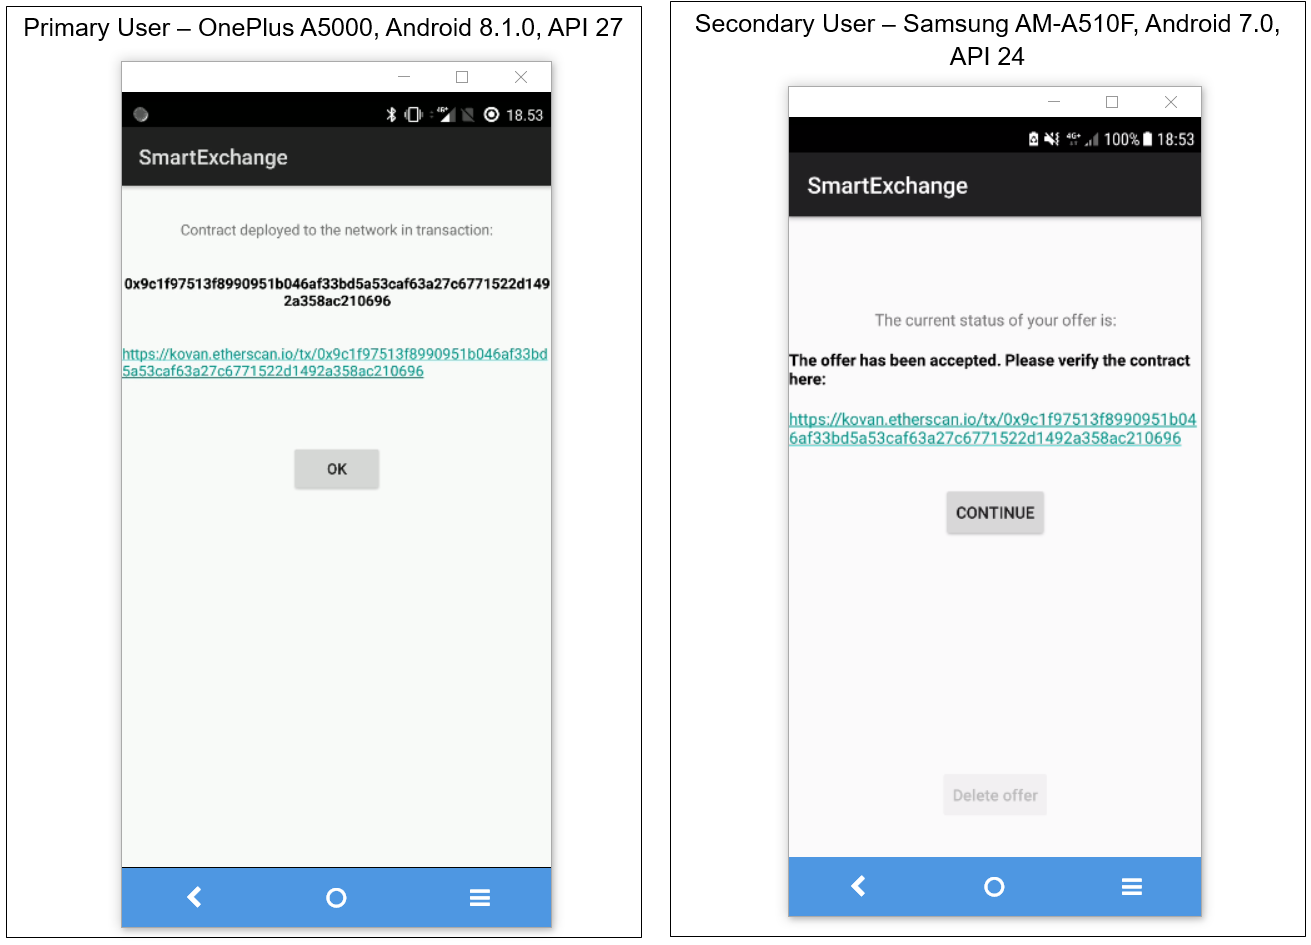
\includegraphics[width=\textwidth]{screenshots/screen091}
    \caption{Screen of both instances of the application, after the smart contract has been deployed to the network. Eve is on the left.}
    \label{fig:screenshot-contract}
\end{figure}
%
%
%
%
%
%%%%%%%%%%%%%%%%%%%%%%%%%%%%%%%%%%%%%%%%%%%%%%%%%%%%%%%%%%%%%%%%%%%%%%%%%%
\subsubsection{Known weaknesses}
The sample scenario demonstrated that the system enables two users to trade Ether and Bitcoin with the use of a smart contract. However, we must note that this scenario was carried out under ``sunny day conditions''. There was no risk of losing any real currency, since the experiment was carried out on a test network. There was no attacker, attempting to disrupt the transaction process and the external services used (Infura, Oraclize, Blockchain.info and Etherscan) were all operational and honest. The two fictitious users were controlled by the developers, thus they had absolute knowledge about the system and were certain about the various features of the application and about the user interface components. Most of these issues were not addressed due to the time constrains, even though some could be solved easily.

We do realise that this is not always the case and any of these conditions can be violated during regular use. In following paragraphs we describe some of the most severe issues of the system. While the system can still be used, as demonstrated above, if exploited, these issues could lead to the system being unusable or funds being lost in the worst case. These issues should be addressed in further development.

\paragraph{Use of only one node}
The system at its current state only uses a single Infura node. The node does not have control over users funds, since the transactions are signed offline (in the Android application). However, the node could still refuse to send a transaction to a network and this way influence the transaction process. Similar issue persists, if the provider goes offline -- no users would be able to make transactions,

While running a single node is sufficient to demonstrate the idea of the prototype, more work should be put into implementing the solution with multiple nodes. In a market-ready version of the application, the centralisation implied by using a single node would pose as a major, business critical drawback.
% 
\paragraph{Use of only one oracle and blockchain explorer}
As noted previously, the system only uses one oracle and one blockchain explorer provider. Similarly as the Infura node, they could prevent transactions from happening, if either of the two goes offline. Additionally, the blockchain explorer and the oracle can also provide counterfeit data to the smart contract. Either of the two could alter the response to the smart contract, altering the balance on the queried account and therefore influence the behaviour of the smart contract. Using the model scenario as an example, if Mike had not transferred the Bitcoin, but instead manipulated the Blockchain.info, that the queried account does have the balance he was supposed to send, then the smart contract would release the funds to him. In similar fashion he could hypothetically manipulate the oracle, yielding the same result.

A solution, where multiple oracles are queried with different blockchain explorers could make it more difficult to execute the above attack.
% 
\paragraph{Unsecured access to the database}
Firebase allows several options how to restrict the read and write access to the database. With the current setup however, anyone who has the database reference string (database URL) can read and write all data in the database. This is obviously not secure, since anyone could retrieve the string from the application source code and flood the database with bogus offers or delete all existing real offers. The access to the database should be limited, so that this malicious activity is prevented. This could be done by only allowing users to change offers they created and only allowing them to create a limited number of offers per hour. This issue needs to be addressed in the further releases of the application.

\paragraph{Database controls the transaction flow}
The current process of making a transaction is tied to the \texttt{offerStatus} codes received from the database. If users do not wish to interact through the database and decide to use another communication channel outside our system, the application should be able to handle this. Currently, however it does not allow to deploy a contract directly and all the transactions need to be created in the database, before they are picked up by the application.

This functionality should be fixed in the application, where users should be able to deploy a smart contract manually (i.e. where the user selling Ether manually enters all the required data).
% 
\paragraph{User interface flaws}
There were no requirements established for the user interface, nor did the user interface undergo any user testing. There are some flaws in the user interface that make the application confusing to use. This was not addressed in this project as it is out of scope, but should be revisited in further development.

Moreover, due to rather complicated transaction process (Figure \ref{fig:arch-ver2-tech}, p. \pageref{fig:arch-ver2-tech}) and importance of carrying out the steps in the correct order to maintain the desired level of security, the user should be presented with a guide upon the first application launch, which would describe the steps and guide the user through the process of making a transaction.

\paragraph{Ether return policy}
In the prototype, user needs to use the temporary address, generate by the application, as the \textit{Import wallet} function has not been implemented. In case the secondary user does not transfer Bitcoin as agreed, the Ether funds would be returned to this temporary address. The application currently does not display private key of this temporary address, therefore the user is not able to access the returned funds. It is possible to use these funds to make another transaction, but the temporary address is lost when the user closes the application. This is an application flaw and should be fix be redesigning the user interface.